% \documentclass[presentation,xcolor={usenames,dvipsnames}]{beamer}
\documentclass[handout,xcolor={usenames,dvipsnames}]{beamer}
% \newcommand{\sketchyhome}{../../../allresesarch/Storage-optimal-optimization/SketchyCGM/aistats}
% \newcommand{\sketchyfigures}{\sketchyhome/figs}
\newcommand{\talks}{.}
%\input \talks/CTUY16-talk-macros.tex
\input \talks/formatting.tex
\input \talks/defs.tex

\graphicspath{{../spectral/img/}{..spectral/}{../adaptive/img/}{../tensor/}{../tensor/figure/}{../projection/}{../projection/figure/}{./}{..figure/}{figures/}}

\mode<handout>
%\mode<presentation>
{
\usetheme{default}
}



\title{High Dimensional Data Analysis With Dependency and Under Limited Memory}

\date{\today} %\textcolor{blue}{Les Houches OSL, March 2019}}
\author[Yiming Sun Cornell. \textit{}]{%
Yiming Sun\\[1ex]
{Cornell University}\\
\vspace{.4in}
Based on joint work with \\
Madeleine Udell (Cornell), Sumanta Basu(Cornell)\\
Yang Guo (UW Madison),  Charlene Luo (Columbia)\\
Joel Tropp (Caltech), Amy Kuceyeski(Cornell University)\\
Yige Li(Harvard University)}

\begin{document}

\begin{frame}
\titlepage
\end{frame}

\section{Multivariate Spectral Density Estimation Under Weak Sparsity}
\begin{frame}{Motivation}
\begin{figure}
\centering 
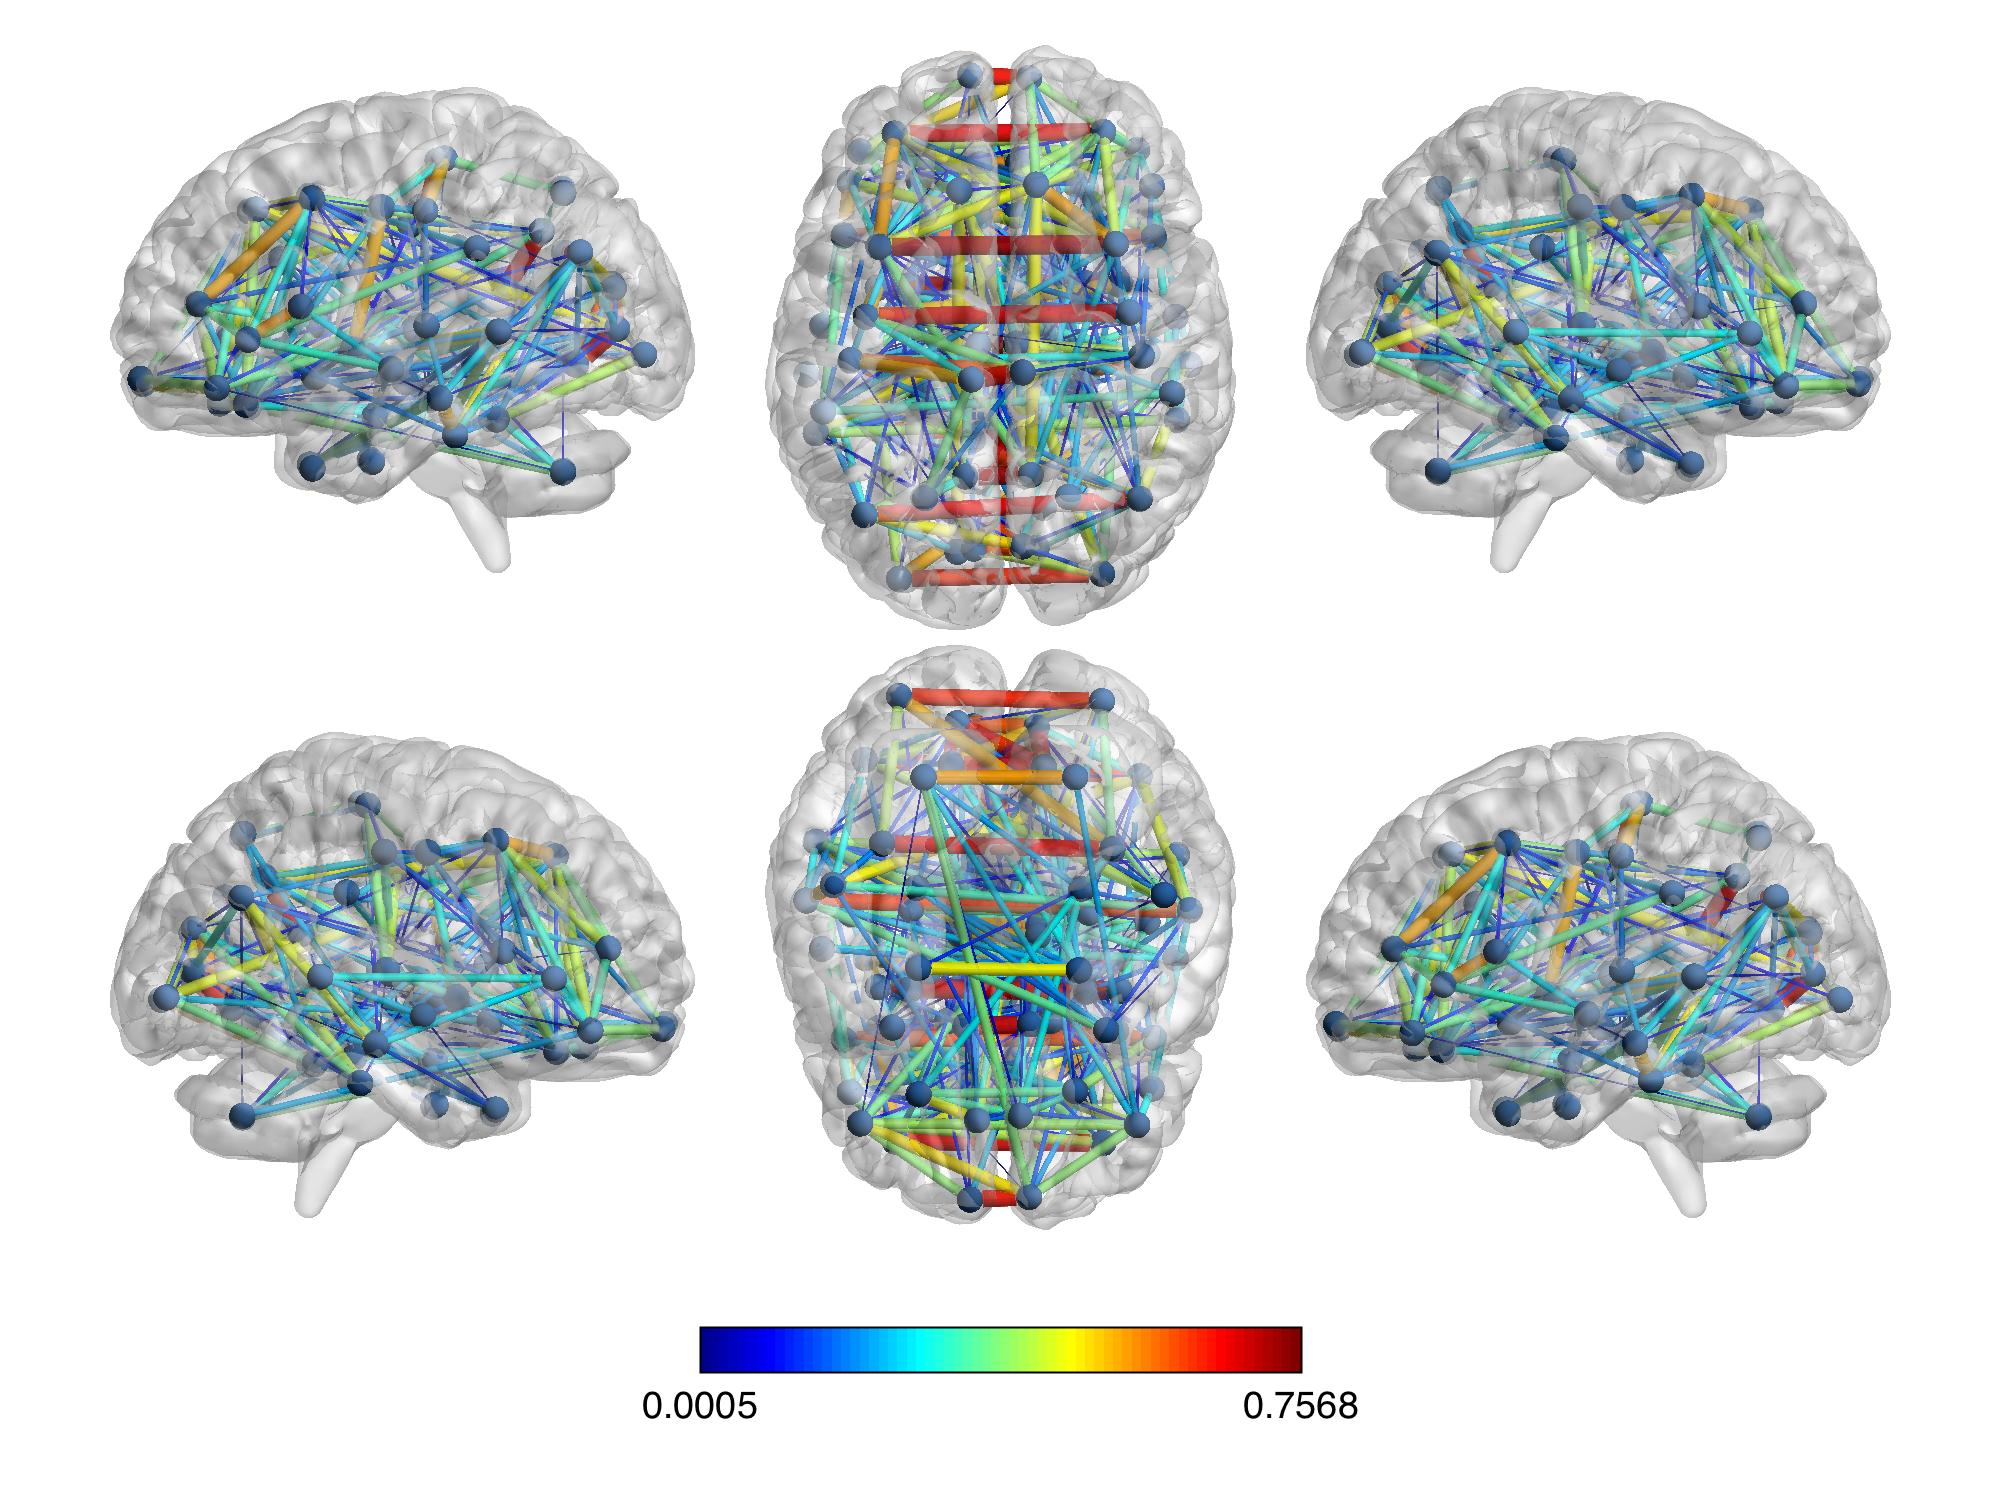
\includegraphics[width=0.6\textwidth]{al_c.jpg}
\caption{Interactions Between Regions in Brain}
\end{figure}
\end{frame}

\begin{frame}{Weakly \& strongly stationary time series}
\begin{definition}[Weak Stationarity]
$p$-variate time series $X$ is weakly stationary, if $\E X_t = \E X_s$ for any $t, s$ and $\Gamma(\ell) := \E X_t X^\top_{t-\ell}$ only depends on the lag $\ell$.  
\end{definition} 
\begin{definition}[Strong Stationarity]
$p$-variate time series $X$ is strongly stationary, if for any sequence $t_1, \cdots, t_n$,  $X_{t_1} \cdots X_{t_n}$ has the same distribution of $X_{t_1+\tau} \cdots X_{t_n+\tau}$ for any integer $\tau$, 
\end{definition}
\end{frame}

\begin{frame}{Gaussian process}
\begin{definition}[Gaussian Process]
$p$-variate time series $X$ is Gaussian process if for any sequence $t_1, \cdots, t_n$,  $X_{t_1} \cdots X_{t_n}$  are jointly Gaussian distributed. 
\end{definition}
For Gaussian process, weak stationarity is equivalent to strong stationarity. 
\end{frame}


\begin{frame}{Spectral density}
Given a weakly stationary $p$-variate time series $X$,  the spectral density at frequency $\omega\in [-\pi,  \pi)$ is defined 
\[
f(\omega) = \sum_{\ell = -\infty} ^\infty \Gamma(\ell) e^{-i\omega \ell} 
\]
where $\Gamma(\ell) = \E X_0X_{-\ell}^\top$.   $X_t$ is independent with $X_s$, $t\neq s$ iff $f_{rs}(\omega) = 0$ for any $\omega$. 
\end{frame}

\begin{frame}{Thresholding estimator under weak sparsity- An example}
Suppose that we have n observation of p-variate Gaussian distribution as follows. 
\[
y_i \overset{i.i.d}{\sim} \mathcal{N}\left(\mu, 
\begin{bmatrix}
\sigma^2_1 & 0 & \cdots & 0\\  
0 & \sigma^2_2 & \cdots & 0\\
\vdots & \vdots & \ddots\\
0 & 0& 0& \sigma^2_p
\end{bmatrix}\right),
\]
$i=1,\cdots, n$. 
\end{frame}

\begin{frame}{An example}
The maximum likelihood estimator for $\mu_j$ is $\bar{y}_j = \frac{1}{n}\sum_{i=1}^n y_{ij}$.   \\ 
{\bf Does not Work Well Under Weak Sparsity} 
\[
\mu \in \left\{\mu \in \mathbb{R}^p, \sum_{j=1}^p |\mu_j|^q \le c_0(p)\right\}. 
\]
for some $0\le q<1$ and $c_0(p)$ measures the weak sparsity. 
\end{frame}


\begin{frame}{Solution : Thresholding}
Suppose $\sigma_i\le B$, define element-wise thresholding operator 
\[
T_\lambda(x) = \begin{cases}
x & |x|\ge  \lambda \\
0 & \text{else}
\end{cases} 
\]. 
Hard thresholding estimator $T_\lambda(\bar{y}_j)$ can be shown asymptotically consistent under weak sparsity where we set 
\[
\lambda \propto B   \sqrt{\frac{\log p}{n}}
\] 
and assume $\lambda\rightarrow 0$. 
\end{frame}

\begin{frame}{Two key ingredients for thresholding}
Two key ingredients under above example assuming weak sparsity. \cite{cai2011adaptive}
\begin{itemize}
\item An element-wise concentration inequality : 
\[
\mathbb{P}( |\bar{y}_j - \mu_j | \ge \eta) \le 2 \exp(-n\eta^2/2\sigma_j^2). 
\]
\item $\sigma_j$ are uniformly bounded.  
\end{itemize}
\end{frame}

\begin{frame}{Shortcomings for hard thresholding}
\begin{itemize}
	\item $\sigma_j$ may variate much
	\item $B$ will appear in the thresholding value making convergence rate slow 
\end{itemize}
\end{frame}


\begin{frame}{Solution: adaptive thresholding}
Simply estimate $\sigma_j$, say with sample standard deviation: 
\[
\hat{\sigma}_j = \sqrt{1/(n-1)\sum_{i=1}^n (y_{ij} - \bar{y}_j)^2}
\]
and replace $B$: $\lambda_j \propto \hat{\sigma}_j \sqrt{\frac{\log p}{n}}$.  Now we can relax constraint in upper bound for $\sigma_j$ and upper bound will not appear in rate of convergence. 
\end{frame}

\begin{frame}{An Similar Example: Covariance Matrix}
\[
y_i \overset{i.i.d}{\sim} \mathcal{N}(0, \Sigma_{p\times p})
\]
{\color{red} Goal:} Estimate $\Sigma$ assuming weak sparsity, $\|\Sigma\|_{1}\le c_0(p)$ .  \cite{bickel2008covariance}
\end{frame}


\begin{frame}{A similar example: covariance matrix}
Estimate the expectation of a vector of length $p^2$:
\[
[(y_1y_1^\top )_{rs}, 1\le r, s\le p]. 
\]
{\color{red} MLE:} $\hat{\Sigma} = \frac{1}{n} \sum_{i=1}^n y_i y_i^\top$.  But we need to perform thresholding.  Remember two ingredients:
\begin{itemize}
\item $\mathbb{P}(|\hat{\Sigma}_{rs} - \Sigma_{rs}|\ge \eta) \le c_1\exp(-c_2n\eta^2)$
\item $\Var((y_1y_1^\top)_{rs}) = \Sigma_{rr}\Sigma_{ss}+\Sigma^2_{rs} \le 2\max_{r=1}^p\Sigma^2_{rr}$
\end{itemize}
Thus \cite{bickel2008covariance} presents an assumption $\max_{r=1}^p\Sigma_{rr}$ is bounded. 
\end{frame}

\begin{frame}{A similar example: covariance matrix}
\red{hard thresholding:} $\lambda_{rs} \propto (\max_{r=1}^p \Sigma_{rr}) \sqrt{\frac{\log p}{n}}$ \\ 
\red{adaptive thresholding:} $\lambda_{rs} \propto \sqrt{\widehat{\Var(y_1y_1^\top)_{rs}}}\sqrt{\frac{\log p}{n}}$
where 
\[
\widehat{\Var(y_1y_1^\top)_{rs}} = \frac{1}{n-1}\sum_{i=1}^n \left[(y_iy_i^\top)_{rs} -  \frac{1}{n} \sum_{i=1}^n (y_iy_i^\top)_{rs} \right]^2
\]
\end{frame}


'

\section{Low Rank Tucker Approximation of a Tensor from Streaming Data}


\begin{frame}{Motivation}
We listed three scenarios for Motivation Borrowed from Professor Udell's Recent Talk
\end{frame}


\newcommand{\stream}{$\T{X}^{(t)} = \T{H}_1 + \cdots + \T{H}_t$}
\newcommand{\all}{$\T{X}^{(T)} = \T{H}_1 + \cdots + \T{H}_T$}
\newcommand{\db}{$\T{X} = \T{H}_1 + \cdots + \T{H}_T$}
\newcommand{\tapx}{$\hat{\T{X}}$}
\newcommand{\skstream}{$\mathcal L(\T{X}^{(t)}) = \mathcal L(\T{H}_1 + \cdots + \T{H}_{t-1}) + \mathcal L(\T{H}_t)$}
\newcommand{\skall}{$= \mathcal L(\T{H}_1 + \cdots + \T{H}_{T-1}) + \mathcal L(\T{H}_T)$}
\newcommand{\skdb}{$\mathcal L(\T{X}) = \mathcal L(\T{H}_1) + \cdots + \mathcal L(\T{H}_T)$}
\newcommand{\skx}{$\mathcal L(\T{X})$}
\newcommand{\skxt}{$\mathcal L(\T{X}^{(T)})$}
\newcommand{\x}{$\T{X}$}


\begin{frame}{Big data, small laptop}

% large database, high latency
% small compute
% can stream data to compute (maybe more than once)

\begin{tikzpicture}
\node[inner sep=3pt] (toaster) at (-4,0)
{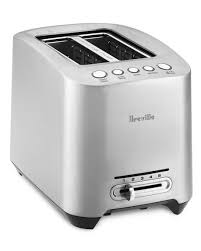
\includegraphics[height=.2\textheight]{toaster.jpeg}};
\node[inner sep=3pt,label=below:\db] (db) at (0,0)
{
\includegraphics[height=.2\textheight]{database.jpeg}};
\node[inner sep=3pt,label=below:\bad{\x}] (laptop) at (5,0)
{
\includegraphics[height=.2\textheight]{laptop.jpeg}};
\draw[->,thick] (toaster.east) -- (db.west)
node[midway,fill=white] {$\T{H}_T$};
\draw[->,thick] (db.east) -- (laptop.west)
node[midway,fill=white] {\bad{\x}};
\end{tikzpicture}

\end{frame}



\begin{frame}{Distributed data}

% many toasters
% toaster has low memory
% limited bandwidth
% can only store/send sketch of data
% privacy angle: don't share Personally Identifiable Toast Information (need no-PITI algorithm)

\begin{tikzpicture}
\node[inner sep=3pt] (toastert) at (-4,0)
{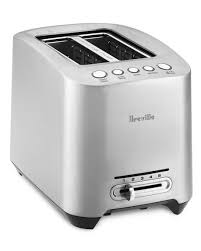
\includegraphics[height=.1\textheight]{toaster.jpeg}};
\node[inner sep=3pt] (toaster1) at (-4,2)
{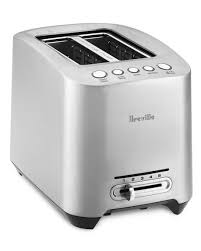
\includegraphics[height=.1\textheight]{toaster.jpeg}};
\node[inner sep=3pt] (toasterT) at (-4,-2)
{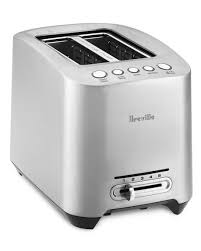
\includegraphics[height=.1\textheight]{toaster.jpeg}};
\node[inner sep=3pt,label=below:\db] (db) at (1.5,0)
{
\includegraphics[height=.17\textheight]{database.jpeg}};
\node[inner sep=3pt,label=below:\bad{\x}] (laptop) at (5.5,0)
{
\includegraphics[height=.17\textheight]{laptop.jpeg}};
\draw[->,thick] (toaster1.east) -- (db.west)
node[midway,fill=white] {$\T{H}_1$};
\draw[->,thick] (toastert.east) -- (db.west)
node[midway,fill=white] {$\T{H}_t$};
\draw[->,thick] (toasterT.east) -- (db.west)
node[midway,fill=white] {$\T{H}_T$};
\draw[->,thick] (db.east) -- (laptop.west)
node[midway,fill=white] {\bad{$\x$}};
\draw[loosely dotted] (toaster1.south) -- (toastert.north);
\draw[loosely dotted] (toastert.south) -- (toasterT.north);
\end{tikzpicture}

\end{frame}

\begin{frame}{Streaming data}

% left arrow toaster right arrow
% toaster has low memory
% $\T{X}^{(t)} = \T{H}_1 + \cdots + \T{H}_t$
% can only store sketch of data
\begin{tikzpicture}
\node[inner sep=3pt,label=below:\bad{\stream}] (toaster) at (0,-2)
{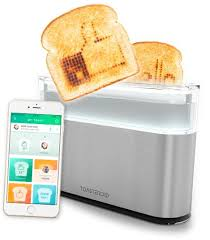
\includegraphics[width=.2\textwidth]{smart-toaster.jpeg}};
\node[inner sep=0pt] (toast) at (0,2)
{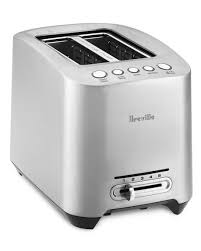
\includegraphics[width=.2\textwidth]{toaster.jpeg}};
\draw[->,thick] (toast.south) -- (toaster.north)
node[midway,fill=white] {$\T{H}_t$};
\node[inner sep=0pt] (start) at (-4,2)
{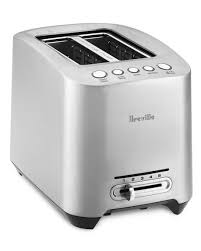
\includegraphics[width=.2\textwidth]{toaster.jpeg}};
\node[inner sep=0pt] (end) at (4,2)
{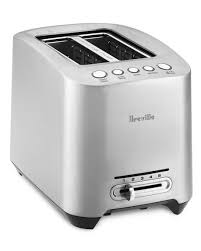
\includegraphics[width=.2\textwidth]{toaster.jpeg}};
\draw[->,thick] (start.east) -- (toast.west);
\draw[->,thick] (toast.east) -- (end.west);
\end{tikzpicture}
\end{frame}

\begin{frame}{Notation}
tensor to compress:
\bit
\item tensor $\T{X} \in \reals^{I_1 \times \cdots \times I_N}$ with $N$ modes
\item sometimes assume $I_1 = \cdots = I_N = I$ for simplicity
\eit

\pause indexing:
\bit
\item $[N] = 1,\ldots,N$
\item $I_{(-n)} = I_1 \times  \cdots \times  I_{n-1} \times   I_{n+1} \times I_N$
\eit

\pause tensor operations:
\bit
\item mode $n$ product: for $\T{A} \in \reals^{k \times I_n}$ ,
$\T{X} \times_n \M{A} \in \reals^{I_1 \times \cdots \times I_{n-1} \times k \times I_{n+1} \times \cdots \times I_N}$ %contracts $\T{A}$ with $\T{B}$ along mode $n$
\pitem unfolding $\M{X}^{(n)} \in \reals^{I_n \times I_{(-n)}}$ stacks mode-$n$ fibers of $\T{X}$ as columns of matrix
\eit
\end{frame}

\begin{frame}{Review of Our Tool: Linear Sketch}
A linear random projection can be represented as a random matrix $\mathbf{\Omega}\in \reals^{d\times k}$, operating on a vector $\mathbf{x}\in \reals^{d}$ or a matrix $\mathbf{X} \in \reals^{m\times d}$ to reduce the dimension:
\begin{equation}
\label{eq:low_dim_mapping}
\begin{aligned}
&\mathbf{x} \in \reals^{n} \rightarrow  \mathbf{\Omega}^\top \mathbf{x} \in \reals^{k} \\
& \mathbf{X} \in \reals^{m\times d} \rightarrow   \mathbf{X}\mathbf{\Omega} \in \reals^{m\times k}. 
\end{aligned}
\end{equation}
\end{frame}

\begin{frame}{Properties Preserved after Projection}
\begin{lem}[\citet{arriaga2006algorithmic}]
	\label{lem:gauss-rp-vector}
	Let $\mathbf{x} \in \reals^d$, assume that the entries in $\mathbf{\Omega}\in \reals^{d\times k}$ are sampled independently from $\mathcal{N}(0, 1)$. Then
	\begin{equation}
	\label{eq:gauss_random_projection}
	\Prob\left((1-\epsilon)\|\mathbf{x}\|^2 \le \left\|\frac{1}{\sqrt{k}} \mathbf{\Omega}^\top \mathbf{x}\right\|\le (1+\epsilon)\|\mathbf{x}\|^2\right)\le 1 - 2e^{-(\epsilon^2-\epsilon^3)k/4}.
	\end{equation}
\end{lem}

\begin{lem}[\citet{halko2011finding}]
	\label{lemma:gauss-rp-matrix}
	Let $\mathbf{X} \in \reals^{m\times d}$, assume that the entries in $\mathbf{\Omega}\in \reals^{d\times (k+p)}$ are sampled independently from $\mathcal{N}(0, 1)$. Then let  $\mathbf{Q}$  
	be the orthonormal matrix  from QR factorization $\mathbf{X\Omega} = \mathbf{QR}$, then 
	\begin{equation}
	\label{eq:gauss_col_preservation}
	\|\mathbf{X} - \mathbf{QQ}^\top \mathbf{X}\|_F \le \left(1+\frac{k}{p-1}\right)^{1/2}\left(\sum_{j>k} \sigma_j^2\right)^{1/2}.
	\end{equation}
\end{lem}
\end{frame}

\begin{frame}{Tucker factorization}

rank $\V{r} = (r_1, \ldots, r_N)$ \textbf{Tucker factorization}
of $\T{X} \in \reals^{I_1 \times \cdots \times I_N}$:
%with $N$ modes, assume dimension $I$ in each mode for simplicity
\beas
\T{X} &=& \T{G} \times_1 \M{U}_1 \cdots \times_N \M{U}_N
=: \llbracket\T{G}; \M{U}_1, \ldots, \M{U}_N \rrbracket
% \\ &=& \sum_{i_1 = 1}^{r_1} \cdots \sum_{i_N = 1}^{r_N} g_{i_1\cdots i_N} \V{u_1}_{:i_1} \times \cdots \times \V{u_N}_{:i_N}
\eeas
where
\bit
\item $\T{G} \in \reals^{r_1 \times \cdots \times r_N}$ is the \textbf{core matrix}
\item $\M{U}_n \in \reals^{I_n \times r_n}$ is the \textbf{factor matrix} for each mode $n \in [N]$
\eit
\pause (sometimes assume $r_1 = \cdots = r_N = r$ for simplicity)

\pause
Tucker is useful for compression: when $N$ is small,
\bit
\item Tucker stores $O(rNI)$ numbers for rank $r^3$ approximation
\item CP stores $O(rNI)$ numbers for rank $r$ approximation
\eit

\end{frame}

\begin{frame}{The sketch}

approximate factor matrices and core:
\bit
\pitem \textbf{Factor sketch} ($\V{k}$).
For each $n \in [N]$,\\
fix random DRM $\M{\Omega}_n \in \mathbb{R}^{I_{(-n)} \times k_n}$
and compute the sketch
\[
\M{V}_n = \M{X}^{(n)}\M{\Omega}_n
\quad \in \reals^{I_n \times k_n}.
\]
\pitem \textbf{Core sketch} ($\V{s}$).
For each $n \in [N]$, \\
fix random DRM $\M{\Phi}_n \in \reals^{I_n \times s_n}$.
Compute the  sketch
\[
\T{H} =\T{X} \times_1 \mathbf{\Phi}_1^\top \cdots \times_N \M{\Phi}_N^\top
\quad \in \reals^{s_1 \times \cdots \times s_N}.
\]
\pitem \emph{Rule of thumb.} Pick $\V{k}$ as big as you can afford, pick $\V{s} = 2\V{k}$.
\pitem define $\left(\T{H}, \mathbf{V}_1, \ldots, \mathbf{V}_N\right) =
\textproc{Sketch}\left(\T{X}; \{\M{\Phi}_n, \M{\Omega}_n\}_{n \in [N]}\right)$
\eit

\end{frame}

\begin{frame}{Low memory DRMs}

factor sketch DRMs are big! {\red{Same size of the tensor}}
\bit \item $I_{(-n)} \times k_n$ for each $n \in [N]$ 
\eit

\bit
\item {\red{Solution:}}  Generate random matrix $\M{A}_n \in \reals^{I_n\times k}$ \citeb{sun2019low}
\[
\label{eq:TRP}
\M{\Omega}:= (\mathbf{A}_1 \odot \cdots \odot \mathbf{A}_N)
\]
\[
\mathbf{A} \otimes \mathbf{B} = \left[
\begin{array}{ccc}
A_{11}\mathbf{B}   & \cdots & A_{1n}\mathbf{B} \\
\vdots & \ddots & \vdots \\
A_{m1}\mathbf{B} & \cdots &   A_{mn}\mathbf{B}
\end{array}
\right].
\]
We let $\mathbf{X} \odot \mathbf{Y}$ denotes the \textit{Khatri-Rao product}, $\mathbf{A} \in \mathbb{R}^{I \times K}, \mathbf{B} \in \mathbb{R}^{J \times K}$, i.e. the "matching column-wise" Kronecker product. The resulting matrix of size $(IJ) \times K$ is given by: 
\begin{equation}\label{khatri-rao}
\mathbf{A} \odot \mathbf{B} = [\mathbf{A}_{(1,.)} \otimes \mathbf{B}_{(1,.)}, \dots, \mathbf{A}_{(K, .)} \otimes \mathbf{B}_{(K,.)}].
\end{equation}
\eit
\end{frame}


\begin{frame}{Two pass algorithm}

\begin{algorithm}[H]
	\caption{Two Pass Sketch and Low Rank Recovery \label{alg:two_pass_low_rank_appro}}
	\textbf{Given:} tensor $\T{X}$,
	DRMs $\{\M{\Phi}_n, \M{\Omega}_n\}_{n \in [N]}$
	with parameters $\V{k}$ and $\V{s} \geq \V{k}$
	\ben
	\item \emph{Sketch.}
	$\left(\T{H}, \mathbf{V}_1, \ldots, \mathbf{V}_N\right) =
	\textproc{Sketch}\left(\T{X}; \{\M{\Phi}_n, \M{\Omega}_n\}_{n \in [N]}\right)$
	\item \emph{Recover factor matrices.} For $n \in [N]$,
	\[
	(\mathbf{Q}_n, \sim) \leftarrow \rm{QR}(\mathbf{V}_n)
	\]
	\item \emph{Recover core.}
	\[
	\T{W} \leftarrow \T{X} \times_1 \M{Q}_1 \cdots \times_N \M{Q}_N
	\] 
	\een
	\textbf{Return:} Tucker approximation
	$\tilde{\T{X}} = \llbracket\T{W}; \M{Q}_1, \ldots, \M{Q}_N \rrbracket$
	with rank $\leq \V{k}$
\end{algorithm}
\pause accesses $\T{X}$  twice: 1) to sketch 2) to recover core

\end{frame}

\begin{frame}{Intuition: one pass core recovery}

%\mnote{$\Phi$s are transposed in this talk compared to paper but I like this notation better}
\bit
\item we want to know $\T{W}$: \\
compression of $\T{X}$ using factor range approximations $\M{Q}_n$
\item we observe $\T{H}$: \\
compression of $\T{X}$ using random projections $\M{\Phi}_n$
\eit
how to approximate $\T{W}$?
\pause
\beas
\T{X} &\approx& \T{X} \times_1 \M{Q}_1 \M{Q}_1^\top \times \cdots \times_N \M{Q}_N \M{Q}_N^\top \\
&=& \left( \T{X} \times_1 \M{Q}_1^\top \times_N \cdots \times \M{Q}_N^\top \right) \times_1 \M{Q}_1 \dots \times_N \M{Q}_N \\
&=& \T{W} \times_1 \M{Q}_1 \dots \times_N \M{Q}_N \\
\underbrace{\T{X} \times_1 \M{\Phi}_1^\top \dots \times_N \M{\Phi}_N^\top}_{\T{H}}
&\approx& \T{W} \times_1 \M{\Phi}_1^\top \M{Q}_1 \times \cdots \times_N \M{\Phi}_N^\top \M{Q}_N \\
\eeas
\pause
we can solve for $\T{W}$: $\V{s} > \V{k}$, so each $\M{\Phi}_n^\top \M{Q}_n$ has a left inverse (whp):% when $s_n \geq k_n$
\[
\T{W} \approx \T{H} \times_1 (\M{\Phi}_1^\top \M{Q}_1)^\dagger \times \cdots \times_N (\M{\Phi}_N^\top \M{Q}_N)^\dagger
\]

\end{frame}

\begin{frame}{One pass algorithm}

\begin{algorithm}[H]
	\caption{One Pass Sketch and Low Rank Recovery}
	\textbf{Given:} tensor $\T{X}$, rank $\V{r} = (r_1, \ldots, r_N)$,
	DRMs $\{\M{\Phi}_n, \M{\Omega}_n\}_{n \in [N]}$
	% \begin{algorithmic}[1]
	% 	\State
	\bit
	\item \emph{Sketch.}
	$\left(\T{H}, \mathbf{V}_1, \ldots, \mathbf{V}_N\right) =
	\textproc{Sketch}\left(\T{X}; \{\M{\Phi}_n, \M{\Omega}_n\}_{n \in [N]}\right)$

	\item \emph{Recover factor matrices.} For $n \in [N]$,
	\[
	(\mathbf{Q}_n, \sim) \leftarrow \rm{QR}(\mathbf{V}_n)
	\]
	% 	\EndFor
	% 	\State
	\item \emph{Recover core.}
	\[
	\T{W} \leftarrow \T{H} \times_1 (\M{\Phi}_1^\top \M{Q}_1)^\dagger \times \cdots \times_N (\M{\Phi}_N^\top \M{Q}_N)^\dagger
	\]  %\Comment{access $\T{X}$}
	% 	\State \Return $\T{W_0}, \mathbf{Q}_1, \cdots, \mathbf{Q}_N$
	% 	\EndFunction
	% \end{algorithmic}
	\eit
	\textbf{Return:} Tucker approximation $\hat{\T{X}} = \llbracket\T{W}; \M{Q}_1, \ldots, \M{Q}_N \rrbracket$
\end{algorithm}
\pause accesses $\T{X}$ only once, to sketch
\source{\citeb{sun2019low}}

\end{frame}


\begin{frame}{Fixed rank approximation}

to truncate reconstruction to rank $\V{r}$, truncate core:
\begin{lem}
	\label{lemma: equivalance_one_pass}
	For a tensor $\T{W}\in \mathbb{R}^{k_1 \times \cdots \times k_N}$,
	orthogonal matrices $\mathbf{Q}_n \in \mathbb{R}^{k_n\times r_n}$,% for $n \in [N]$,
	\[
	\llbracket \T{W}\times_1 \mathbf{Q}_1 \cdots \times_N \mathbf{Q}_N \rrbracket_\mathbf{r} =
	\llbracket \T{W} \rrbracket_\mathbf{r} \times_1 \mathbf{Q}_1 \cdots \times_N \mathbf{Q}_N,
	\]
	where $\llbracket \cdot \rrbracket$ denotes the best rank $\V{r}$ Tucker approximation.
\end{lem}
\pause
$\implies$ compute fixed rank approximation using, \eg, HOOI on (small) core approximation $\T{W}$

\end{frame}


\begin{frame}{Tail Energy}
For each unfolding $\mathbf{X}^{(n)}$,
define its $\rho$\textit{th tail energy} as
\[
(\tau_\rho^{(n)})^2 := \sum_{k>\rho}^{\min(I_n,I_{(-n)})} \sigma_{k}^2(\mathbf{X}^{(n)}),
\]
where $\sigma_{k}(\mathbf{X}^{(n)})$ is the $k$th largest singular value of $\mathbf{X}^{(n)}$.
\end{frame}

\begin{frame}{Guarantees for two pass}
\begin{thm}[\citeb{sun2018tensor}]
	\label{thm:low_rank_err_two_pass}
	Sketch the tensor $\T{X}$ using a Tucker sketch with parameters $\V{k}$
	using DRMs %$\mathbf{\Omega}_n$, $n \in [N]$,
	with i.i.d. Gaussian $\mathcal N(0,1)$ entries.
	Then the approximation $\hat{\T{X}}_2$ computed with the two pass method \ref{alg:two_pass_low_rank_appro}
	satisfies
	\begin{equation*}
	\mathbb{E}\| \T{X} - \hat{\T{X}}_2 \|_F^2  \le  \min_{1\le \rho_n<k_n-1}
	\sum_{n=1}^N \left(1+\frac{\rho_n}{k_n-\rho_n-1}\right)(\tau^{(n)}_{\rho_n})^2.
	\end{equation*}
\end{thm}
\end{frame}


\begin{frame}{Guarantees for one pass}

\begin{thm}[\citeb{sun2018tensor}]
	Sketch $\T{X}$ with Gaussian DRMs of parameters $\V{k}$, $\V{s} \geq 2\V{k}+1$.
	Form a rank $\V{r}$ Tucker approximation $\hat{\T{X}}$
	using the one pass algorithm.
	Then
	\begin{equation*}
	\mathbb{E}\| \T{X} - \hat{\T{X}} \|_F^2  \le  (1+\Delta) \min_{1\le \rho_n<k_n-1}
	\sum_{n=1}^N \left(1+\frac{\rho_n}{k_n-\rho_n-1}\right)(\tau^{(n)}_{\rho_n})^2
	\end{equation*}
	where $\Delta = \max_{n=1}^N k_n / (s_n-k_n-1)$
\end{thm}
\end{frame}


\begin{frame}{Comparison to other methods in pseudo optimality}
\bit 
\item HOSVD and ST-HOSVD is pseudo optimal with factor $N$:
\begin{equation}
\begin{aligned}
& \| \T{X}-\llbracket \T{X} \rrbracket _{\mathbf{ST-r}}\|_F \le  \sqrt{\sum_{n=1}^N (\tau^{(n)}_{r_n})^2} \le \sqrt{N} \|\T{X}-\llbracket \T{X} \rrbracket _{\mathbf{r}}\|_F, 
\end{aligned}
\end{equation}
\eit 

\bit 
\item Set $\V{k} = 2\V{r}+1$ and $\V{s} = 2\V{k}+1$,  and use truncated QR factorization to get $\M{Q}\in \reals^{I_n\times r_n}$ from factor sketch. 
\begin{equation}
\begin{aligned}
& \| \T{X}- \hat{\T{X}}_2 |_F \le  \sqrt{\sum_{n=1}^N (\tau^{(n)}_{r_n})^2} \le \sqrt{2N} \|\T{X}-\llbracket \T{X} \rrbracket _{\mathbf{r}}\|_F. 
\end{aligned}
\end{equation}
\eit 
\end{frame}

\begin{frame}{Different DRMs perform similarly}
\begin{columns}
	\centering
	\begin{column}{0.3\textwidth}
		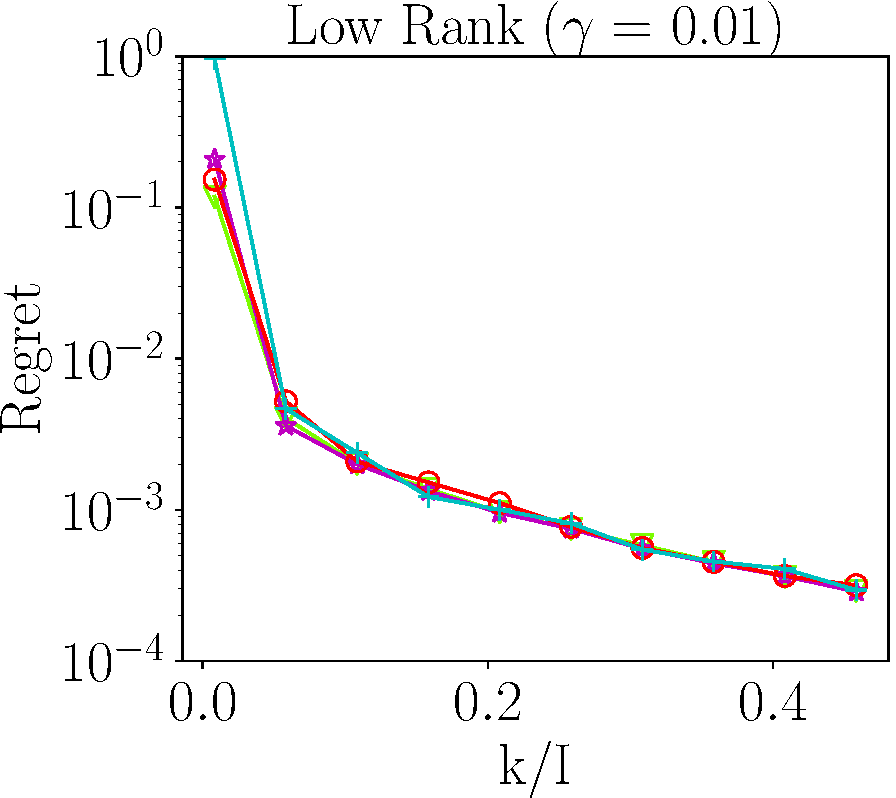
\includegraphics[scale = 0.25]{fig2_lk_lnoise_600.pdf}
	\end{column}
	\begin{column}{0.3\textwidth}
		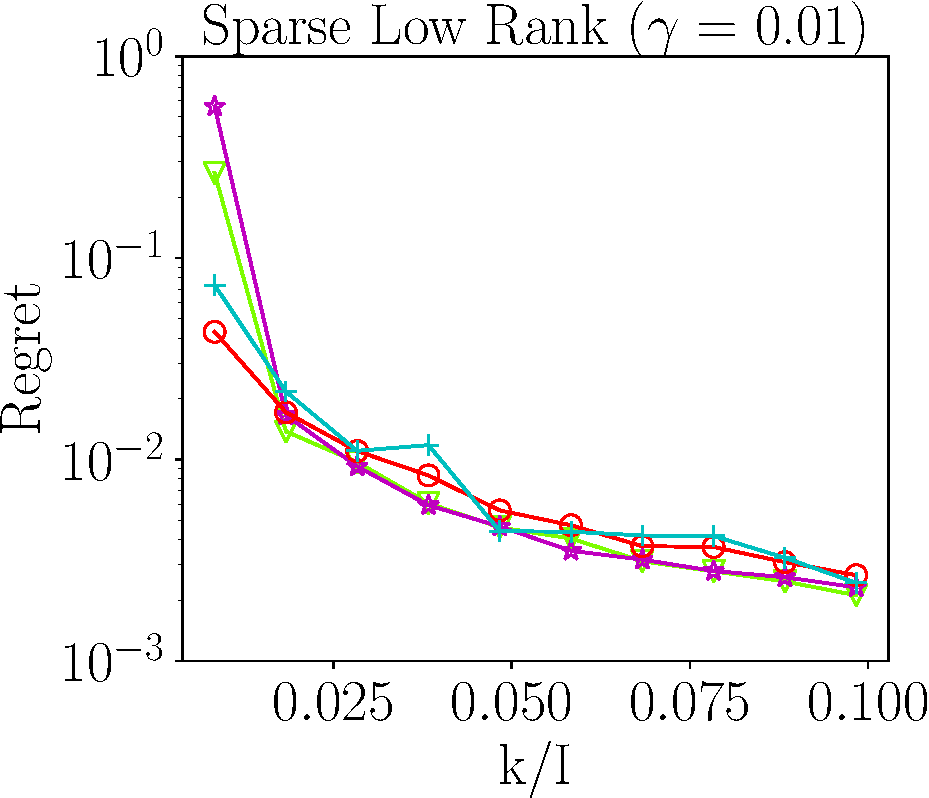
\includegraphics[scale = 0.25]{fig2_slk_lnoise_600.pdf}
	\end{column}
	\begin{column}{0.3\textwidth}
		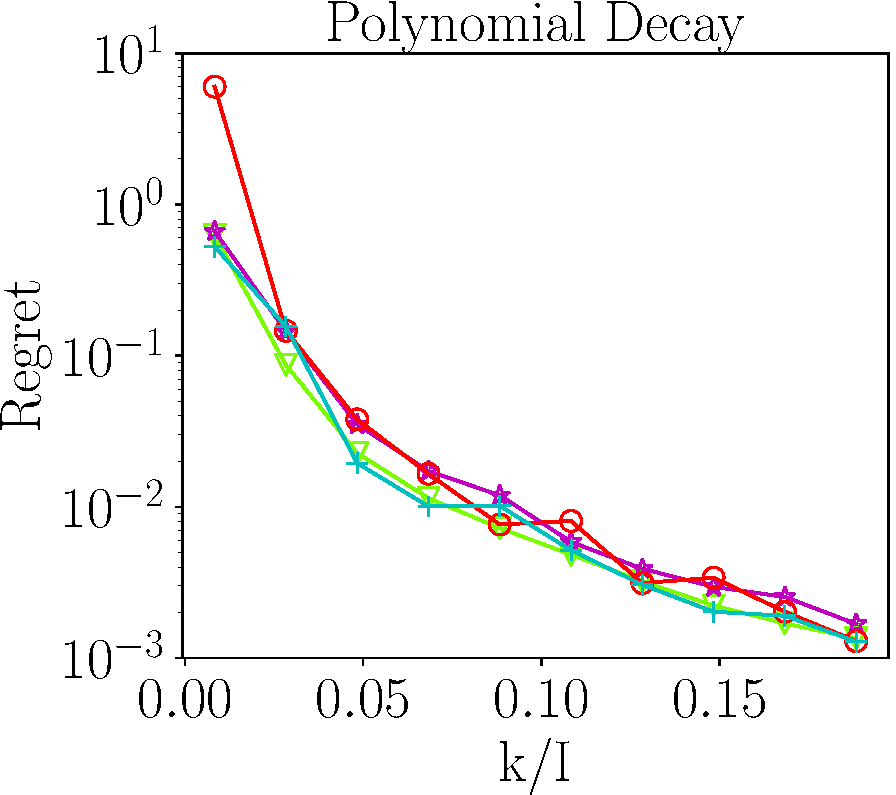
\includegraphics[scale = 0.25]{fig2_spd_600.pdf}
	\end{column}
\end{columns}
\begin{columns}
	\centering
	\begin{column}{0.3\textwidth}
		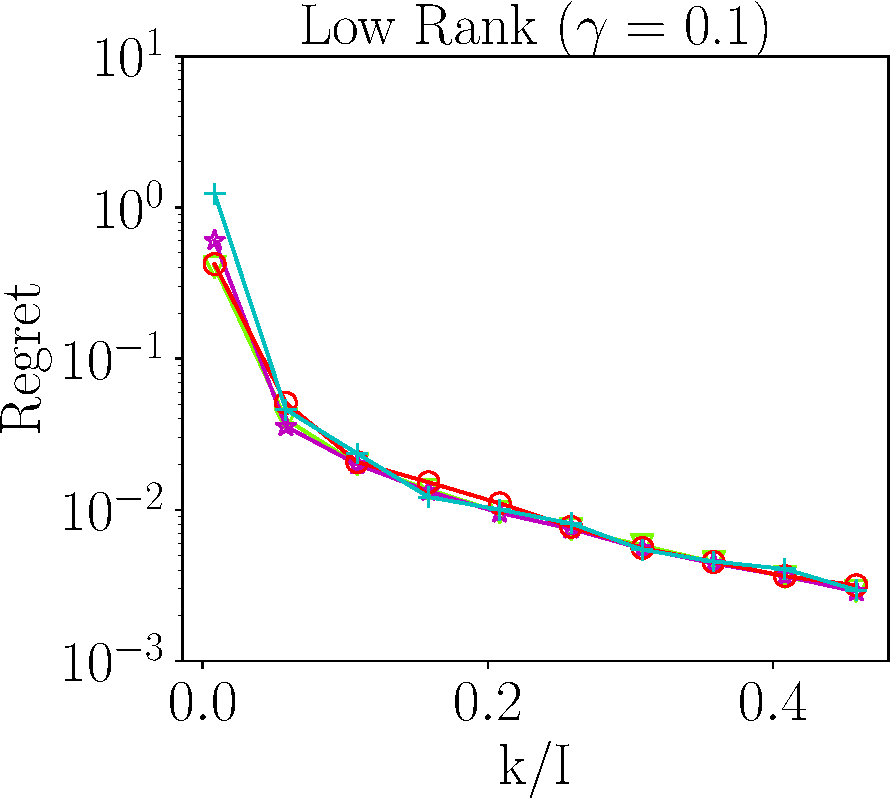
\includegraphics[scale = 0.25]{fig2_lk_mnoise_600.pdf}
	\end{column}
	\begin{column}{0.6\textwidth}
		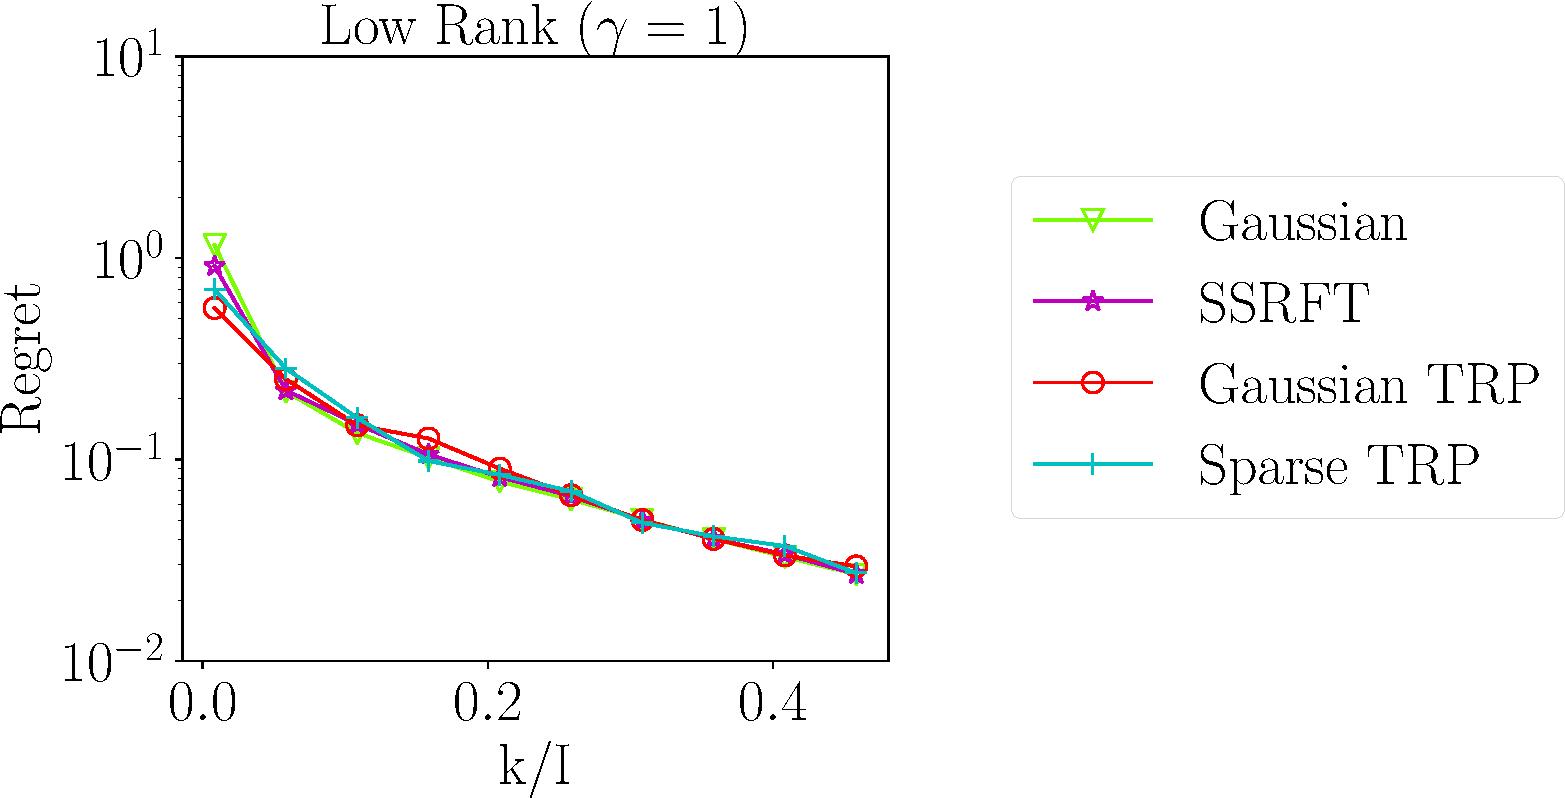
\includegraphics[scale = 0.25]{fig2_lk_hnoise_600.pdf}
	\end{column}
\end{columns}

\comment{Synthetic data, $I = 600$ and $\mathbf{r} = (5,5,5)$. $k/I = .4 \implies$ 20$\times$ compression. }

\end{frame}

\begin{frame}{Video scene classification}
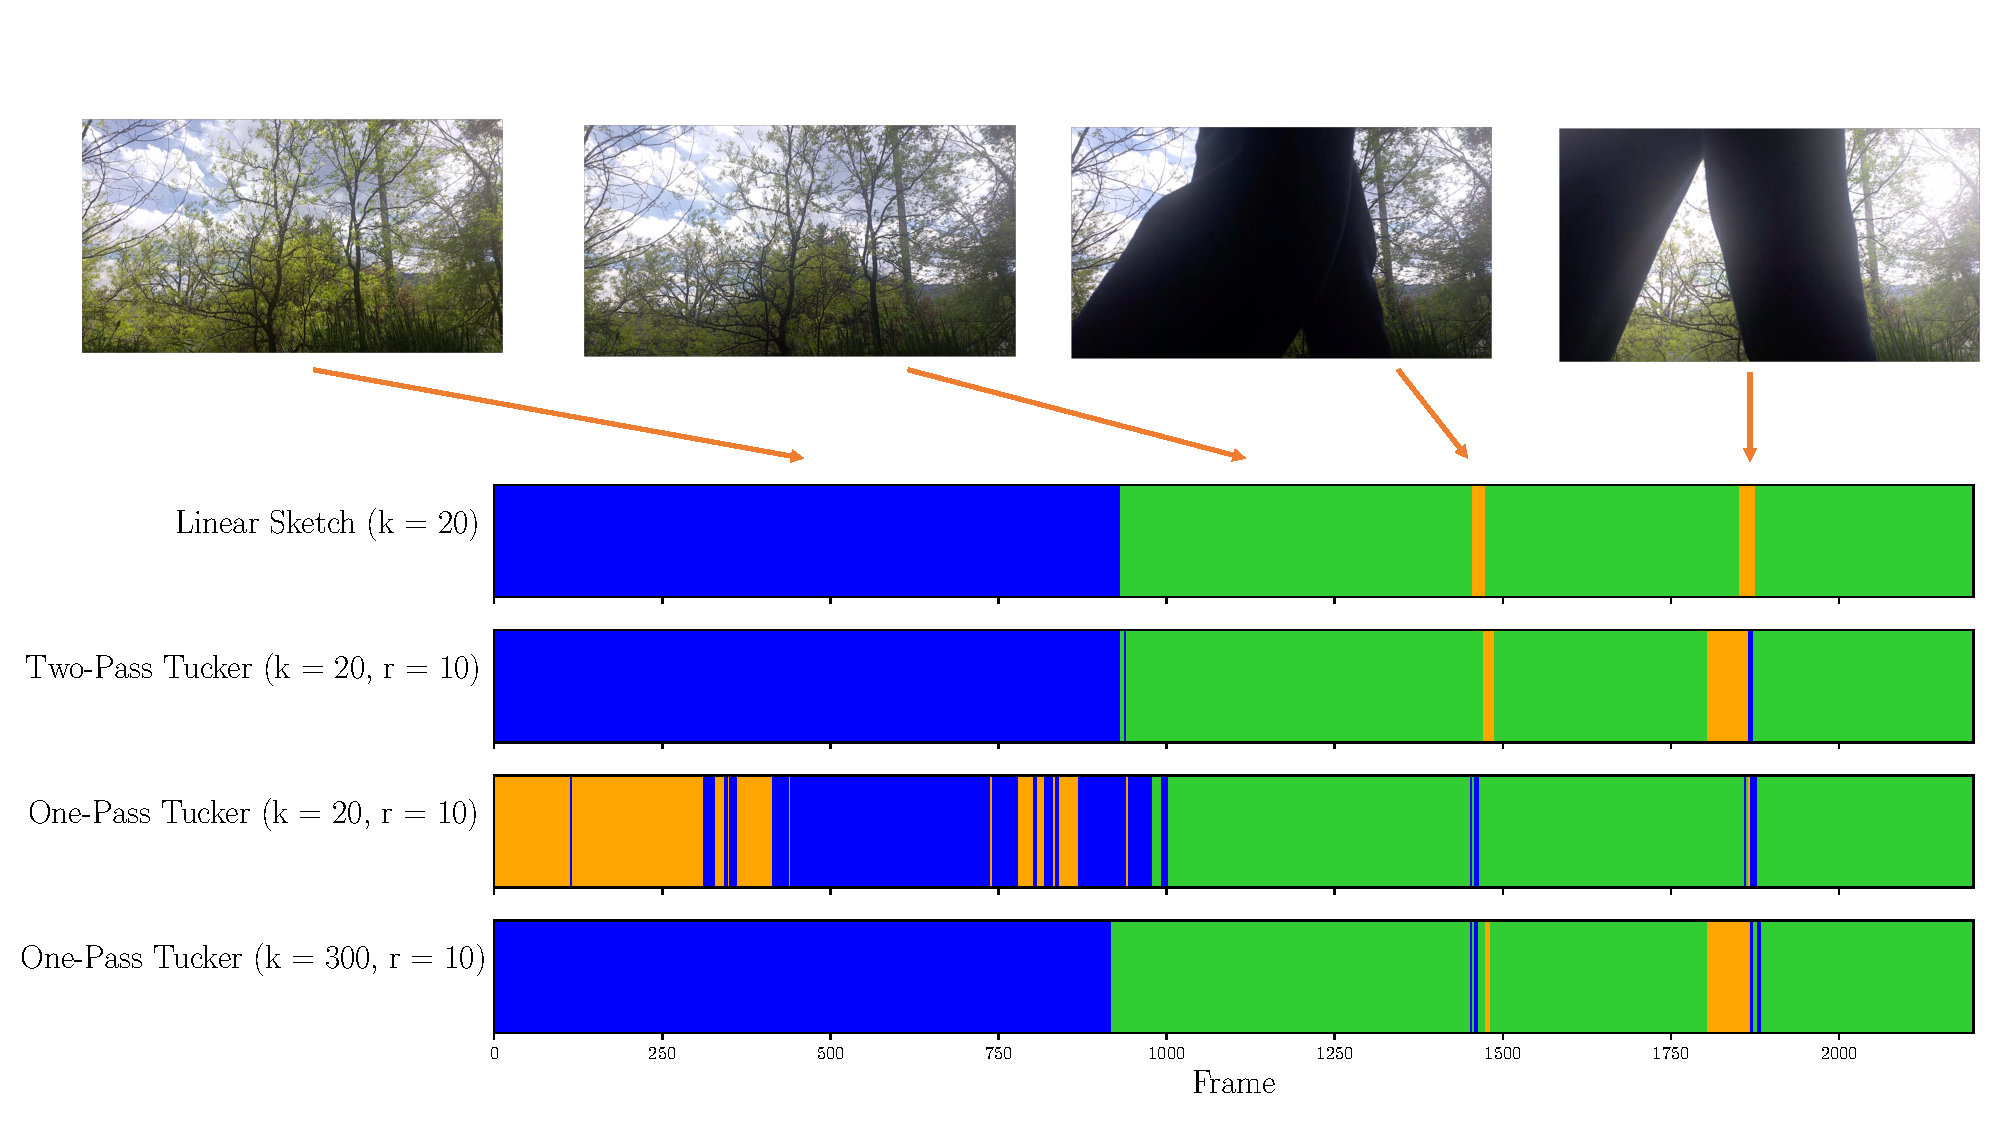
\includegraphics[width=\textwidth]{\figures/video_classification_result.pdf} \\

\comment{Video data $2200 \times 1080 \times 1980$.
	Classify scenes using $k$-means on:
	1) linear sketch along the time dimension $k = 20$ (Row 1);
	2) The Tucker factor along the time dimension, computed via our two pass (Row 2) and one pass (Row 3) sketching algorithm $(r,k,s) = (10,20,41)$.
	3) The Tucker factor along the time dimension, computed via our one pass (Row 4) sketching algorithm $(r,k,s) = (10,300,601)$.
}
\end{frame}


\begin{frame}{Property of tensor random projection}
\red{Preserve Pair-wise Distance}:
Fix $\mathbf{x} \in \reals^{\prod_{n=1}^N d_n}$. Generate random matrix 
\[
\M{\Omega}= (\mathbf{A}_1 \odot \cdots \odot \mathbf{A}_N)
\]
\begin{thm}
	Fix $\mathbf{x} \in \mathbb{R}^{\prod_{n=1}^N d_n}$.
	Form a TRP and $\textup{TRP}_T$ of order $N$ with range $k$
	composed of independent matrices with independent columns
	whose entries are mean zero, variance one, fourth moment $\Delta$, and within each column every pair of elements has covariance zero.
	Then
\begin{equation}
\begin{aligned}
& \E \left\| \frac{1}{\sqrt{k}}\M{\Omega}^\top \mathbf{x} \right\|^2 = \|\mathbf{x}\|^2  \\
& \var(\|\textup{TRP}(\mathbf{x})\|^2) = \frac{1}{k}(\Delta^N-3)\|\mathbf{x}\|_4^4 + \frac{2}{k}\|\mathbf{x}\|_2^4 
\end{aligned}
\end{equation}
\end{thm}
\end{frame}



\section{A Small Example to Connect Two Researches}






\bibliographystyle{plainnat}
\bibliography{biblio1,biblio2,biblio3,biblio4}
\end{document}
